\documentclass[10pt,conference,compsocconf]{IEEEtran}

\usepackage{hyperref}
\usepackage{graphicx}	% For figure environment


\begin{document}
\title{Determining Aspects of Personality from Transcript of Speech}

\author{
  Aryan Ahadinia, Saba Nasiri, Shahrzad Javidi\\
  \texttt{\{aryan.ahadinia, saba.nasiri, shahrzad.javidi\}@epfl.ch}\\
  \textit{EPFL}
}

\maketitle

\begin{abstract}

\end{abstract}

\section{Introduction}



\section{Literature Review}\label{sec: Literature Review}

Language psychology highlights that word choice is influenced not only by meaning but also by psychological factors such as emotions, relational attitudes, power dynamics, and personality traits. As Tausczik and Pennebaker noted, “Words and language [...] are the very stuff of psychology [...] the very medium by which cognitive, personality, clinical, and social psychologists attempt to understand human beings” \cite{Tausczik2010}. Building on this foundation, integrating sociolinguistics with automated text analysis techniques enables the inference of personality traits from written texts \cite{Mairesse2007, Oberlander2006, Minamikawa2011, Gill2009, Luyckx2008}.

Recent advancements in artificial intelligence, particularly in natural language processing and deep learning, have further refined the ability to predict personality traits from social media and other natural language data \cite{Vinciarelli2014}. Techniques like Recurrent Neural Networks (RNNs), Gated Recurrent Units (GRUs), and Long Short-Term Memory (LSTM) networks have been widely used for this purpose \cite{Majumder2017}. For instance, RNNs combined with LSTM, GRU, and Bi-LSTM have effectively captured relationships between sentences in datasets like MBTI, with LSTM models showing the best performance \cite{Hernandez2017}. Hierarchical models using recurrent layers have also been effective in analyzing social media text for detecting Big Five traits \cite{Xue2018}. Transfer learning methods, such as pre-trained BERT models, have been used for multitask prediction of personality and emotions, simplifying the process of working with diverse datasets \cite{Li2021}. In conversations, RNNs combined with Hidden Markov Models (HMMs) have been applied to analyze turn-taking and dialogue exchange for personality detection \cite{Su2016}. Deep learning methods, including LSTM, Bi-LSTM, and GRU, have also demonstrated strong performance in predicting personality traits in languages like Indonesian Bahasa \cite{Jeremy2021}. On LinkedIn, a study of 275 profiles showed that extroversion could be reliably inferred based on self-expression in users’ profiles \cite{VandeVen2017}.

While there is a lot of research on predicting personality traits from text, much less work has been done on predicting IQ. One big reason for this is that it is very hard to find datasets that include both writing samples and IQ scores. Stylometry, which is usually used to identify authors, has recently been explored as a new way to estimate a person’s IQ by looking at the quality and vocabulary of their writing. This method moves away from identifying authors and focuses on understanding cognitive abilities, showing that analyzing text can help measure intelligence \cite{Hendrix2017}. Our work is different because, unlike previous studies that analyze carefully written text, we focus on text transcribed from video content. This text reflects more natural, spontaneous language use, making our approach distinct and suited to studying IQ in real-world contexts. Additionally, due to ethical risks, which we will discuss in the next phase, our study is limited to working only with text.

\newpage

\section{Proposed Methodology}\label{sec: Proposed Methodology}

In this project an end-to-end trainable model is proposed for predicting the target variables. The training procedure is in two stages. In the first stage, a pretrained language model with frozen weights is used for generating embeddings for the texts and then a model is trained for predicting the target variables. In the second stage, the language model and the predictor are subjected to fine-tuning using an augmented dataset.

\subsection{Model Architecture}\label{sec: Model Architecture}

The architecture of the model is illustrated in figure \ref{fig:model_arch} in a glance. In the first step, a numerical embedding of the text is generated using a pretrained language model (LM). Depending on the LM, the final representation of the text can be considered as the sequence mean, \texttt{[CLS]} representation of BERT models, or \texttt{<s>} representation of LLaMa models, which are capturing the overall context of the text. After generating a representation for the input text, it is concatenated with the side information vector. The result of this concatenation is considered as the initial representation associated to a sample.

The initial representation is feeded into a feed-forward multi-layer perceptron network with depth of $d_s$ to generate a secondary embedding. Afterward, a separated network with depth of $d_i$ transforms the secondary embedding into the predictions values. This two phase architecture is designed for capturing the correlations between the target variables. The first network is shared between all predictions, but in contrast, the second network is trained independently for each target variable.

\begin{figure}[ht]
    \centering
    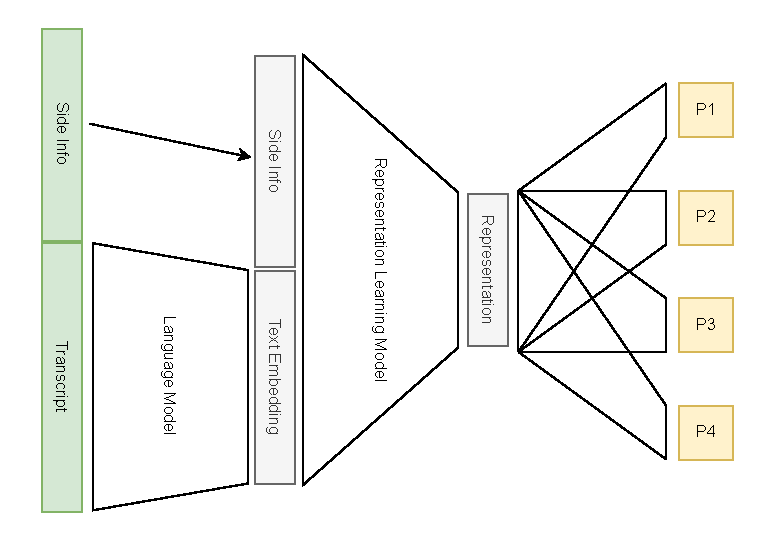
\includegraphics[width=1\linewidth]{assets/model_arch.pdf}
    \caption{Overall architecture of the model. The colored rectangle are associated with internal vector representations.}
    \label{fig:model_arch}
\end{figure}

\subsection{Data Augmentation}\label{sec: Data Augmentation}

Since there is a limited amount of labeled data, it is necessary to use data augmentation methods to increase the training set size. An important criteria in such textual data augmentation is sentiment preservation.

\subsubsection{Back Translation}\label{sec: Back Translation}

\subsubsection{Noise Injection}\label{sec: Noise Injection}

\subsubsection{Masking Methods}\label{sec: Masking Methods}

\subsection{Training}\label{sec: Training}



\subsection{Fine-tuning}\label{sec: Fine-tuning}

Using the augmented dataset and the trained model in the first stage, the model can be fine-tuned now. The regression model's parameters remains fully trainable, however, in contrast, the language model is not fully fine-tuned but parameter efficient fine-tuning methods are employed.

\section{Experiments}\label{sec: Experiments}



\section{Conclusion}\label{sec: Conclusion}



\section*{Acknowledgment}



\bibliographystyle{IEEEtran}
\bibliography{literature}

\end{document}
